\documentclass{sig-alternate-05-2015}
\usepackage{hyperref}
\hypersetup{
    colorlinks=true,
    linkcolor=blue,
    filecolor=magenta,      
    urlcolor=cyan,
}

\begin{document}
\tracingall


\title{Final Report}

\subtitle{\textbf{Team: Dragon Police}}

\numberofauthors{3} 
\author{
\alignauthor
Tyler Coy\\
       \affaddr{Washington State University Vancouver}\\
       \email{tyler.coy@wsu.edu}
\alignauthor
Ty Crabtree\\
       \affaddr{Washington State University Vancouver}\\
       \email{crabtreee.tyler@gmail.com}
\alignauthor Angatvir Sanghera\\
       \affaddr{Washington State University Vancouver}\\
       \email{angatvir.sanghera@wsu.edu}
 }



\maketitle
\section{Introduction}
This project implements a web browser interface that allows users to search and perform queries on a collection of databases. These queries can be performed on the databases: \textit{dinosaurs}, \textit{Super Famicom games}, and\textit{ MMORPG games}. The users are prompted to choose a specific database to index. The interface is constructed to allow users to parse the databases for specific data and information. The user will be able to modify their search through various search engine mechanics. The main focus of interface prompts users to enter specific search terms that are related to the distinct database the user chose to index. Correlating data will be returned and displayed to the user. The primary emphasis of the search engine is to allow users to search for terms within a database; the search finds and return corresponding tuples that matches or relates to the user's search term, and this information is ranked and displayed to the user through the user interface.

\subsection{Software and Modules}
The search engine and indexer of this project is written in Python3. This project utilizes modules that are compatible with Python3 to aid the functionality of the web browser. The project is using the Whoosh query package \cite{Whooshquery}, Whoosh multifield package \cite{Whooshquery}, indexer package \cite{indexer}, and Whoosh's file storage packages \cite{filestorage}. Items being returned are ranked using the TF-IDF \cite{rankmethod} method. The ranking algorithm is also derived from the Whoosh package. This project manages the databases by implementing Whoosh \cite{whoosh} and Sqlite \cite{sql}. The module Flask is implemented For the web framework. This project also uses the modules \textit{mtranslate}\cite{mtranslate}, defaultdict, and \textit{PyDictionary}\cite{PyDictionary} for features pertaining to languages.


\subsection{Overview of Features}
There are specialized features that we chose to enhance and improve the user experience when searching the databases. A specialized feature was to accept multiple languages when searching database. This feature is constructed by importing the \textit{mtranslate}\cite{mtranslate} module. The \textit{mtranslate}\cite{mtranslate} module resembles Google's translate API. The mtranslate module is free opposed to Google's translate API. The next feature that is implemented is the display of images on the interface. This overall enhances the aesthetic of the website. Much of the website consists of plain text. Adding images adds a contrast to the rest of the page, aiding the user experience. Another implemented feature allows links to be click-able, after clicking one of these links the user will be directed to the link's address. This adds a pragmatic use to the interface. This allows this web browser to supplement other web browsers. Another feature shows message prompts within their relative interface boxes (the term \textit{search} will appear within the search-box). This is another aspect that aids the user interface. This adds simplicity to the design of the web browser. Another feature that has been implemented is individual scrolling option for tuple information. This ensures that all the tuples appear the same size, users may scroll if the information within a tuple is larger than what is displayed in the tuple box. A previous button allows users to search for the searched term they last used. Another  feature allows the user to set limits on the number of tuples return. The project also implements a ranking algorithm to display information in an organized manner. The returned tuples will be ranked and returned with the TF-IDF method. This will enhance readability to the browser. Similar tuples will ideally be presented next to one another. The features and the ranking are discussed in more detail below.

\subsection{Translation}
 This project implements a free API package named \textit{mtranslate}\cite{mtranslate}API works by inputting an HTML request that has the text to be translated and what language it is going to be translated to. Once the request is entered an XML page is returned containing the data translated into the specified language.Then using the XML we extract the data using python. This API also allows detection of the inputted language so we can use the detection to specify what language we are going to translate into English. This API was a module designed to emulate Google's translate feature; providing a near ideal implementation of a translation feature.The languages tested and accepted for search terms are English, Hindi, Russian, Mandarin, and French. For example, the same word in two different languages such as, \textit{jurassic} and the french equivalent \textit{jurassique} will return the same tuples to the interface. There are certain caveats with the translation API. Not all words in one language will have an equal translation of the word in another language. Certain words simply have no translation in a foreign language. These caveats are in the minority of possibilities while using the translation API. The accepted languages are not limited to the tested languages. We used Google's translate function to check and test the mtranslate module. The word \textit{super} translated to Hindi is used in a search shown in \textit{Figure 1}.
 ~
\begin{figure}[h]
\center
\fbox{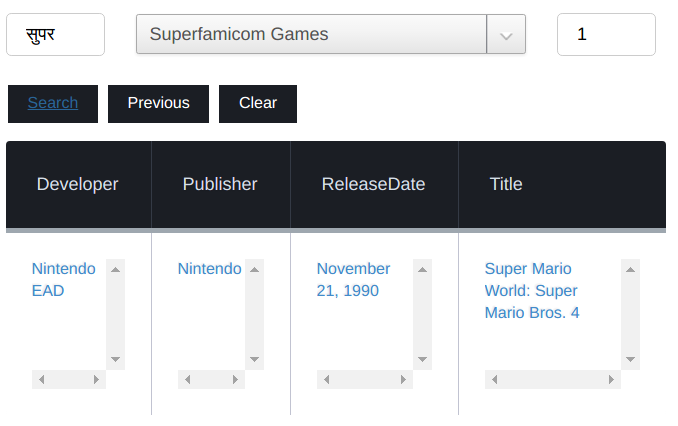
\includegraphics[scale=0.32]{translate.png}}
\caption{Example translation.}
\center
\end{figure}
~
\\
\subsection{Image Implementation}
 This feature consists of grabbing and displaying images on the user interface.  Only tuples that contain images will be displayed to the user. Also, if there is an image category and no image for a specific tuple, the user will be prompted a message saying there is no image found. This feature aids the overall aesthetic of the interface. Without this image implementation, the interface would primarily consist of text. This would be subjectively boring and plain for the user. Allowing images to be presented to the user provides a a mixture of images and text for the user, a subjectively more appealing layout for the user. The layout and appearance of the web browser was taken into account for this feature. An example image can be shown being displayed on the interface in \textit{Figure 2}. 
 ~
\begin{figure}[h]
\center
\fbox{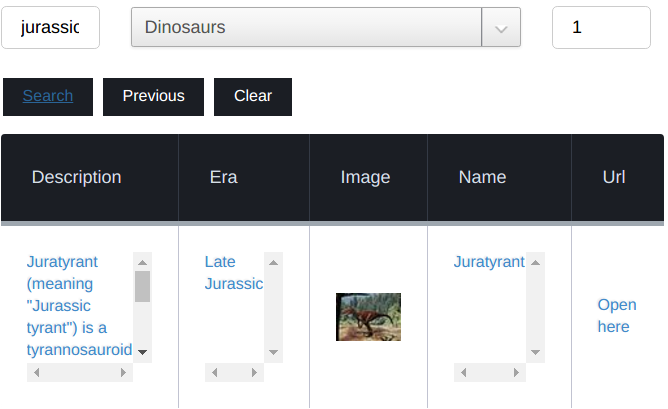
\includegraphics[scale=0.32]{Images.png}}
\caption{Example image parse.}
\center
\end{figure}
~
 
\subsection{Links to an External Website}
The interface has an implementation click-able links for URLS that guid the user to an external website. The user can choose to visit the Wikipedia page that contains information for a specific tuple. This provides a utilitarian aspect to the project. This feature in combination with the other implemented features can help a user traverse Wikipedia within a specific set of parameters. This feature provides an alternative way to traverse Wikipedia. The queries condense the databases to the relevant terms, and the click-able links the user to traverse related pages quickly. This feature supplements the overarching idea of this project; to quickly find relevant and pertinent information through specific queries. Allowing users to utilize the web browser in a variety of methods increases long-lasting appeal. The links can be seen in \textit{Figure 2}.  
 
 \subsection{Limit Tuples}
 Generic search terms may provide hundreds of tuples. This may be overwhelming for a user. To counteract this, the interface implements an optional limit for the tuples displayed. By entering a numerical value the user can set an upper bound for their searches. The user can also choose to ignore this feature (all relevant tuples will be displayed by default). The numerical value of the amount of tuples returned to the interface is also displayed to the user. If the user puts a limit that exceeds the relevant data returned, all relevant data will be returned (which is under the limit set by the user). The interface will provide a prompt for the user instructing how many tuples are returned, educating the user that their search did not return the amount of tuples equal to their the maximum limit value. The amount of tuples will be displayed to the user. The number of tuples returned are not guaranteed to be the same as the limit. For example if the user sets a limit to \textit{1000} and the search term is \textit{Linux} and the database is \textit{dinosaurs}; the results will be far less than the \textit{1000} tuple limit, the tuple limit won't be reach since the search term is unrelated to the database. However, the amount of tuples will always be returned. This can be seen in \textit{Figure 1} and \textit{Figure 2} with the limit being set to \textit{1}.
 
 \subsection{Dynamic Prompts }
  This feature displays dynamic user prompts. Within the interface boxes, such as the search and limit box, the dynamic prompt provides information to the user to instruct the user how to interact with the interface. Terms such as \textit{search} will be located within the search box until a user enters their own search term. The same dynamic prompt will appear for the \textit{limit} section. When the user enters information to search for, this prompt dynamically providing clarity to the user. An example of these prompts can be seen in \textit{Figure 3}.
  ~
\begin{figure}[h]
\center
\fbox{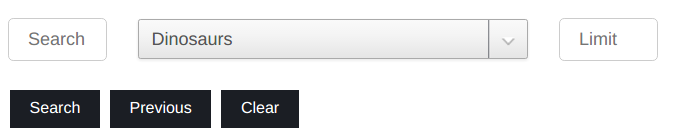
\includegraphics[scale=0.33]{prompts.png}}
\caption{Example prompts.}
\center
\end{figure}
~


 \subsection{Search Clicked Words }
  Tuples within the databases contain various text information. This may be a description of a tuple, title, or other similar data. The user can choose to click any word and that word is then used as the next search term. For example the user sees the word \textit{Triassic} appear in a tuple on the interface. The user can choose to click the word and \textit{Triassic} is used as the next term. There are certain exceptions to this. Links are not searched, this is generally counter-intuitive to the user. Other than links, all other text in the database is searchable. 
  
  \subsection{Scrollable Text Bars  }
  To add congruency between databases scrollable text bars have been added. Text within tuples have a scrolling bar that allows a user to read long sections of text by scrolling. This allows for all text boxes to be the same size. Our databases parses for different information, and this was our method of adding congruency to the pages. \textit{Figure 4} depicts the scrolling text bar. These appear right next to the the text in the tuple. Hovering a mouse over the tuple will highlight the tuple further extenuating the scrollable text bars. 
  
    ~
\begin{figure}[h]
\center
\fbox{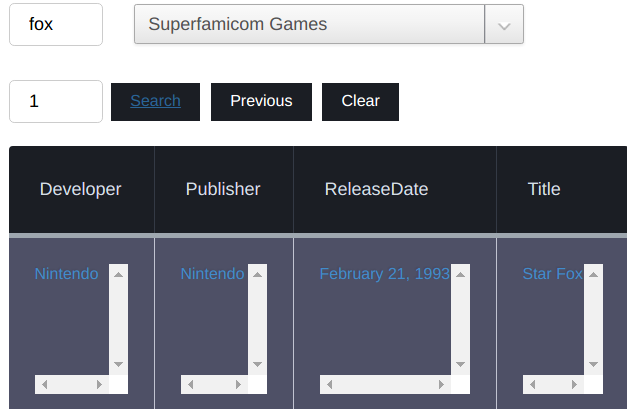
\includegraphics[scale=0.27]{Scroll.png}}
\caption{Example prompts.}
\center
\end{figure}
~
 
  \subsection{Previous Button  }
  To add more functionality to the interface we gave the user the ability search using previously searched items. A list is made of of search terms. A user can then hit the previous button to traverse this list backwards. Potentially a user could press the previous button multiple times in a row and the list will continue to be traversed back towards the first searched term. Upon reaching the first searched term the previous button will simple perform a new search using the first term.
  
 \subsection{Raking}
 The TF-IDF ranking is used. TF-IDF is an acronym for term frequency-inverse document frequency. The TF-IDF algorithm weighs the user's search word assign the importance to that keyword based on the number of times it appears in the document. The most pertinent information is returned first, towards the top of the interface, and the least pertinent information appears towards the bottom of the interface. The implementation of this ranking algorithm came from the Whooh module which had a built in TF-IDF ranking system. The TF-IDF relies on the most frequently occurring terms (these are considered to be the high term frequency terms). Certain frequent words such as; 'the', 'them', 'this', and 'a'  appear frequently within documents. The TF-IDF also determines how unique a word may be. This method looks also at how infrequently the word appears (this is inverse document frequency). By making a comparison of term frequency and uniqueness returns a value for TF-IDF. Words that score a high TF-IDF score occur the most frequently in a unique manner (excluding meaningless terms).
\\
\section{Search Engine}
The search engine for the web browser allows users to specifically tailor searches. The user can modify their queries in a variety of possibilities: by searching for precise terms, providing a tuple limit, selecting specific databases, and clicking on almost any searched word. A user may use a combination of these features to enhance one singular search. \textit{Figure 5} shows a search for the word \textit{Roi} (which is French for \textit{king}) in the database \textit{Super Famicon Games} with a limit set to \textit{2}. The TF-IDF ranking can also be seen in \textit{Figure 5}. The word \textit{king} appears multiple times in the first tuple listed and only once in the second tuple listed. 
 ~
\begin{figure}[h]
\center
\fbox{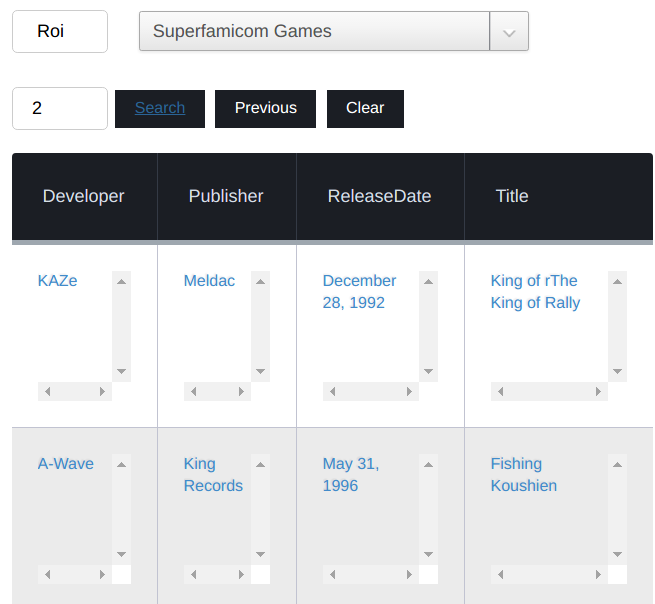
\includegraphics[scale=0.29]{search.png}}
\caption{Example query.}
\center
\end{figure}
~
\\
These features can be utilized in conjunction with one another. In another example, by clicking on the term \textit{1991} a search is performed on this term. After the search is performed (within the database \textit{Super Famicon Games}) the user is prompted that 47 results were returned. This example is shown in \textit{Figure 6}. This example depicts the limit tuple feature and search clicked words feature being used in unison. 
 ~
\begin{figure}[h]
\center
\fbox{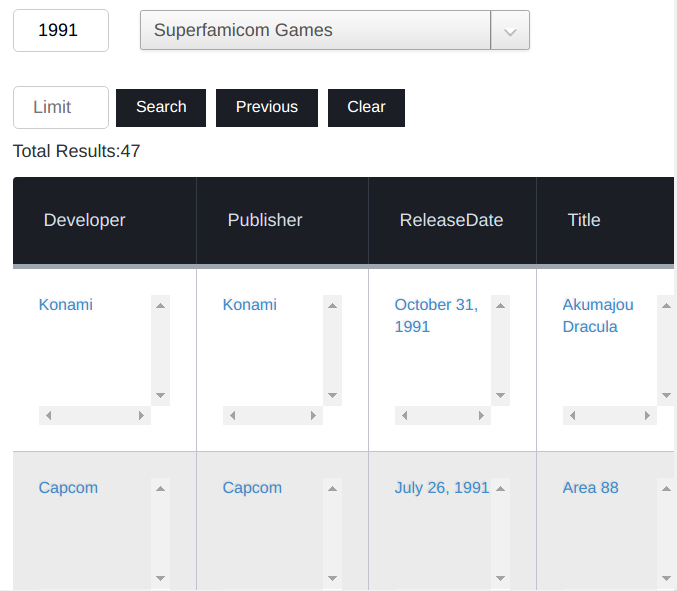
\includegraphics[scale=0.29]{limitClick.png}}
\caption{Example click search.}
\center
\end{figure}
~

 The search engine is designed to be clear, concise, and effective. The intention is only to add features to aid the user, none that needlessly complicate the interface. The goal of the interface is to alleviate work for the user. These specialized features work harmoniously with one another to aid the user.  


\iffalse
\subsection{Citations}
Citations to articles \cite{bowman:reasoning,
clark:pct, braams:babel, herlihy:methodology},
conference proceedings \cite{clark:pct} or
books \cite{salas:calculus, Lamport:LaTeX} listed
in the Bibliography section of your
article will occur throughout the text of your article.
You should use BibTeX to automatically produce this bibliography;
you simply need to insert one of several citation commands with
a key of the item cited in the proper location in
the \texttt{.tex} file \cite{Lamport:LaTeX}.
The key is a short reference you invent to uniquely
identify each work; in this sample document, the key is
the first author's surname and a
word from the title.  This identifying key is included
with each item in the \texttt{.bib} file for your article.

The details of the construction of the \texttt{.bib} file
are beyond the scope of this sample document, but more
information can be found in the \textit{Author's Guide},
and exhaustive details in the \textit{\LaTeX\ User's
Guide}\cite{Lamport:LaTeX}.

This article shows only the plainest form
of the citation command, using \texttt{{\char'134}cite}.
This is what is stipulated in the SIGS style specifications.
No other citation format is endorsed or supported.
\fi


\section{Conclusion}

This project is complete with full functionality. The group did encounter some obstacles during development. The translation package that our group originally decided to use was the Google API. Google charges for translations, so we were forced to find an alternative solution. To fix this we decided to use Microsoft's Bing translation API. Unfortunately, we also found that Microsoft is also charging for the use of their API. Eventually, this search led us to the free translation API we are currently using, the mtranslate module. The group heavily focused on the user interface. Our databases were quite different, with different information. However, we designed an interface that has congruency. All data with text has a scrollable bar in the text box. This limits the size of these boxes (allowing all tuple boxes to be the same size). This also adds a similar look to all of the databases. 

We feel that we have managed our time well since we have accomplished many of our goals, especially some of the harder tasks. Overall the project has been very successful in many aspects. The group is impressed with the usefulness of the \textit{mtranslate}\cite{mtranslate} module. Displaying images makes the browser look ascetically pleasing. The dynamic prompts are a simple touch that improve the design. This clears up website while being functional. The tuple limit adds some helpful functionality. This helps fine tune what is displayed on the interface; this has been extremely useful for testing and will most likely be useful to the users as well. The click-able links are a pragmatic touch. The scrollable text boxes add congruency. The previous button increases the possibilities for user interaction with the interface. 

Overall, the group feels content with the finished project. In many regards we attempted to go above and beyond the expectations set for this project; in many we have succeeded at the expectations and goals set for ourselves. The group is fairly confident at the resilience of the features we have implemented. We feel this has been a successful project.  


\section{Future Work}
The project has been successful, but can still be built upon. In the future, more databases can easily be added to the collection. This is easiest way to expand the project into a more useful web browser. Expanding upon the interface would be an effective aspect for improvement. The interface could be embellished and elaborated upon. The current state of the interface is clean and consistent; the interface could be changed to be subjectively more entertaining. All of the information is pulled from Wikipedia's API. Expanding upon the databases through Wikipedia's API would be easy and add substance to the web browser. Including another website's API to parse and store with the collection of databases would help this web browser exceed the capabilities of Wikipedia in some aspects. Integrating more originality into the project is a focal point for future expansion. This project has many excellent features, yet is limited in information to access. Expanding upon the interface and databases with varied API's would be possibilities for future work. 



\bibliographystyle{abbrv}
\bibliography{references}
\appendix
\section{Introduction}
\section{Software and Modules}
\section{Overview of Features}
\subsection{Translation}
\subsection{Image Implementation}
\subsection{Links to an External Website}
\subsection{Limit Tuples}
\subsection{Dynamic Prompts}
\subsection{Search Clicked Words}
\subsection{Scrollable Text}
\subsection{Previous Button}
\subsection{Ranking}
\section{Search Engine}
\section{Conclusion}
\section{Future Work}



\end{document}
